\documentclass[]{article}
\usepackage[utf8]{inputenc}
\usepackage[slovak]{babel}
\usepackage{graphicx}
\usepackage{float}

\newcommand\ImageItem[2][]{%
	\hfill\raisebox{\dimexpr-\height+\baselineskip}{\includegraphics[#1]{#2}}\hfill~}

\begin{document}
	
	
	\title{TIN - Zbierka príkladov}
	\date{\today}
	
	\maketitle
	\newpage
	\tableofcontents
	\newpage
	
	\section{Chomského hierarchia}
	
	\begin{figure}[H]
		
\includegraphics[width=\textwidth]{tasks/chomsky/task1.png}
	\end{figure}
	
	\begin{figure}[H]
		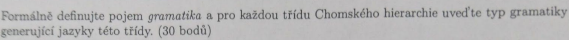
\includegraphics[width=\textwidth]{tasks/chomsky/task2.png}
	\end{figure}

	\section{Regulárne jazyky}
	
	\begin{figure}[H]
		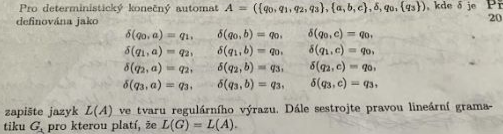
\includegraphics[width=\textwidth]{tasks/regularne/task1.png}
	\end{figure}
	
	\begin{figure}[H]
		
\includegraphics[width=\textwidth]{tasks/regularne/task2.png}
	\end{figure}
	
	\begin{figure}[H]
		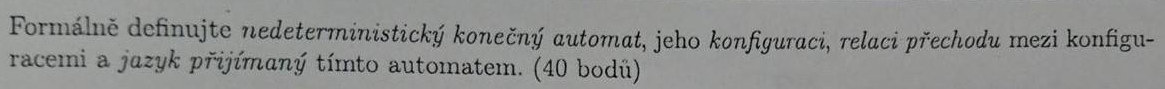
\includegraphics[width=\textwidth]{tasks/regularne/task3.png}
	\end{figure}
	
	\begin{figure}[H]
		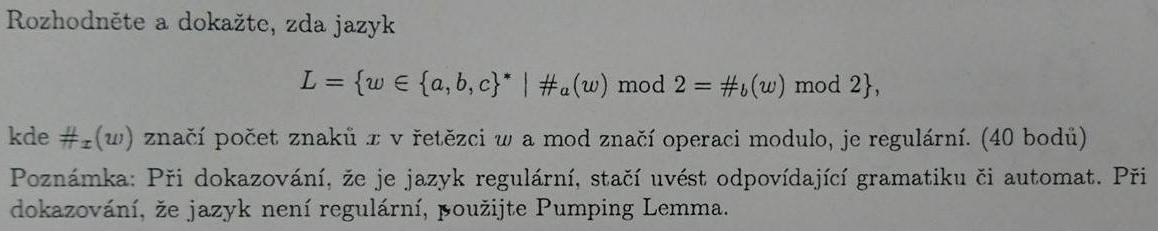
\includegraphics[width=\textwidth]{tasks/regularne/task4.png}
	\end{figure}
	
	\begin{figure}[H]
		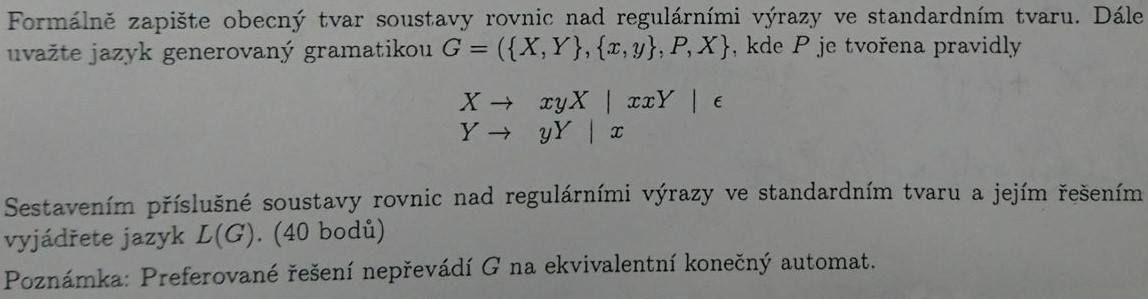
\includegraphics[width=\textwidth]{tasks/regularne/task5.png}
	\end{figure}
	
	\begin{figure}[H]
		
\includegraphics[width=\textwidth]{tasks/regularne/task6.png}
	\end{figure}
	
	\begin{figure}[H]
		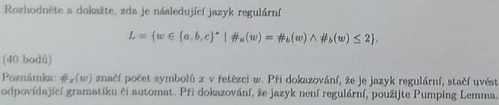
\includegraphics[width=\textwidth]{tasks/regularne/task7.png}
	\end{figure}
	
	\begin{figure}[H]
		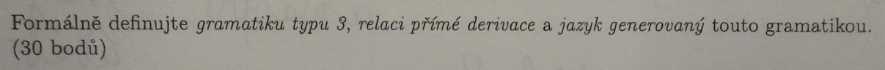
\includegraphics[width=\textwidth]{tasks/regularne/task8.png}
	\end{figure}
	
	\begin{figure}[H]
		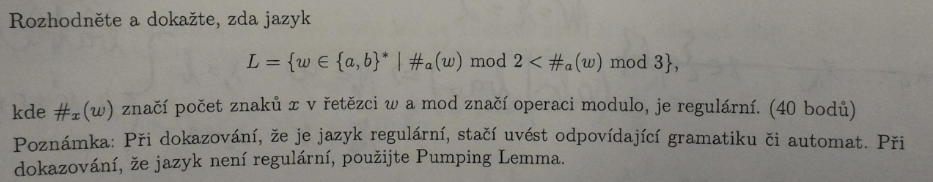
\includegraphics[width=\textwidth]{tasks/regularne/task9.png}
	\end{figure}

	\section{Bezkontextové jazyky}
	
	\begin{figure}[H]
		
\includegraphics[width=\textwidth]{tasks/bezkontextove/task1.png}
	\end{figure}

	\begin{figure}[H]
		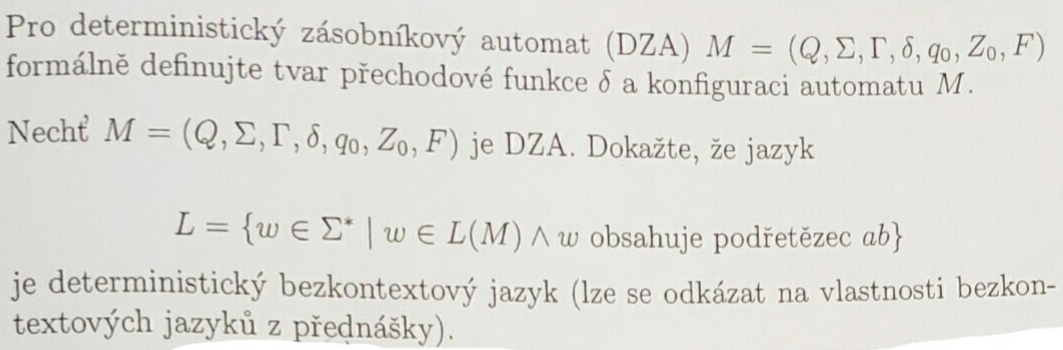
\includegraphics[width=\textwidth]{tasks/bezkontextove/task2.png}
	\end{figure}
	
	\begin{figure}[H]
		
\includegraphics[width=\textwidth]{tasks/bezkontextove/task3.png}
	\end{figure}
	
	\begin{figure}[H]
		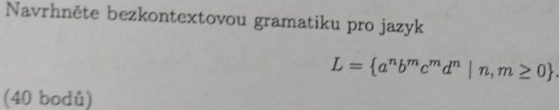
\includegraphics[width=\textwidth]{tasks/bezkontextove/task4.png}
	\end{figure}
	
	\begin{figure}[H]
		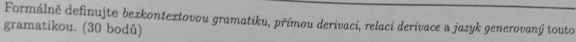
\includegraphics[width=\textwidth]{tasks/bezkontextove/task5.png}
	\end{figure}
	
	\begin{figure}[H]
		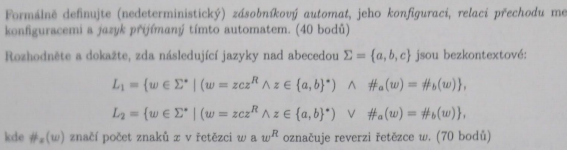
\includegraphics[width=\textwidth]{tasks/bezkontextove/task6.png}
	\end{figure}
	
	\begin{figure}[H]
		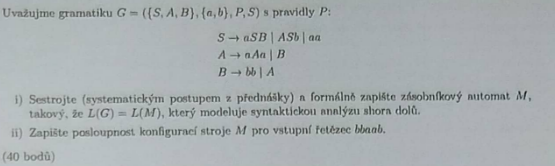
\includegraphics[width=\textwidth]{tasks/bezkontextove/task7.png}
	\end{figure}
	
	\begin{figure}[H]
		
\includegraphics[width=\textwidth]{tasks/bezkontextove/task8.png}
	\end{figure}

	\begin{figure}[H]
		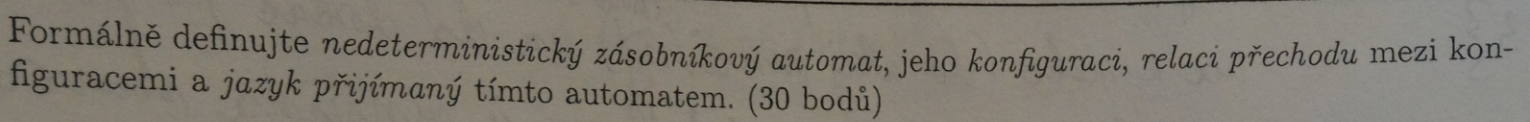
\includegraphics[width=\textwidth]{tasks/bezkontextove/task9.png}
	\end{figure}
	
	\begin{figure}[H]
		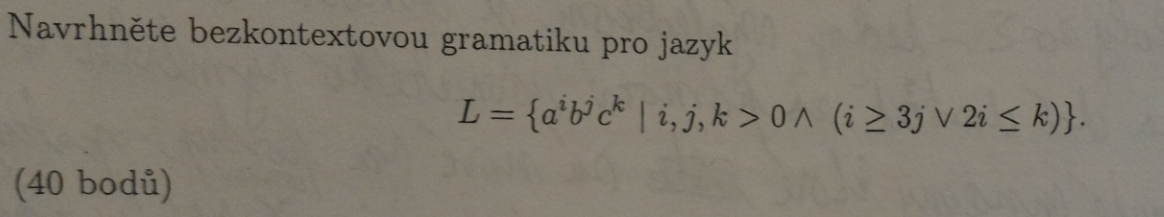
\includegraphics[width=\textwidth]{tasks/bezkontextove/task10.png}
	\end{figure}
	
	\begin{figure}[H]
		
\includegraphics[width=\textwidth]{tasks/bezkontextove/task11.png}
	\end{figure}
	
	\begin{figure}[H]
		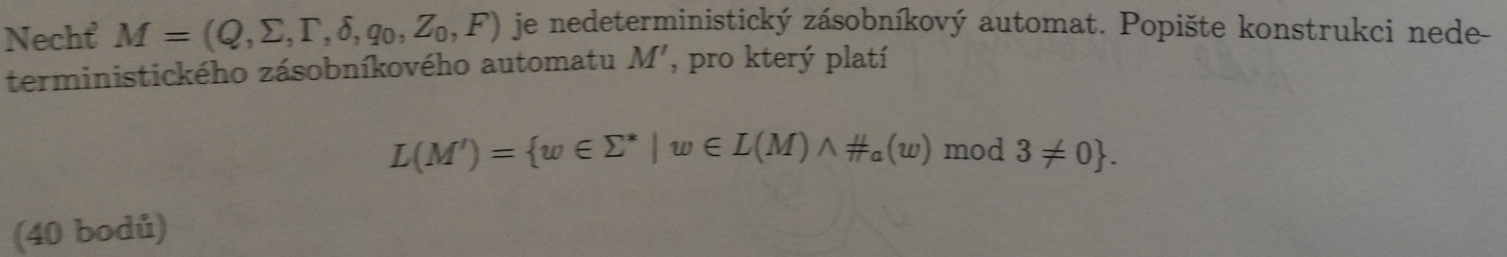
\includegraphics[width=\textwidth]{tasks/bezkontextove/task12.png}
	\end{figure}
	
	\begin{figure}[H]
		
\includegraphics[width=\textwidth]{tasks/bezkontextove/task13.png}
	\end{figure}
	
	\begin{figure}[H]
		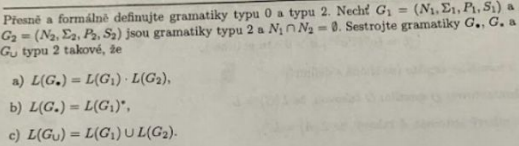
\includegraphics[width=\textwidth]{tasks/bezkontextove/task14.png}
	\end{figure}

	\section{Algoritmy}
	
	\begin{figure}[H]
		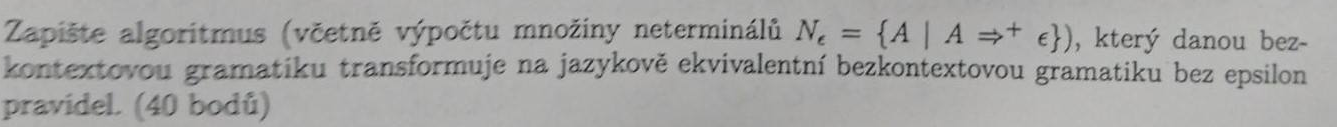
\includegraphics[width=\textwidth]{tasks/algoritmy/task1.png}
	\end{figure}
	
	\begin{figure}[H]
		
\includegraphics[width=\textwidth]{tasks/algoritmy/task2.png}
	\end{figure}
	
	\begin{figure}[H]
		
\includegraphics[width=\textwidth]{tasks/algoritmy/task3.png}
	\end{figure}
	
	\section{Uzáverové vlastnosti}
	
	Definicia, co je to uzavretost triedy jazykov. Dokaz neuzavretosti deterministickych bezkontextovych jazykov na operacie prienik a zjednotenie. Zadana binarna relacia, dokazat, ze je uzavrena. $L1 \circ L2 = \{uv \mid u \in L1 \land v \in L2 \land \vert uv \vert \leq 5\}$.
	
	\begin{figure}[H]
		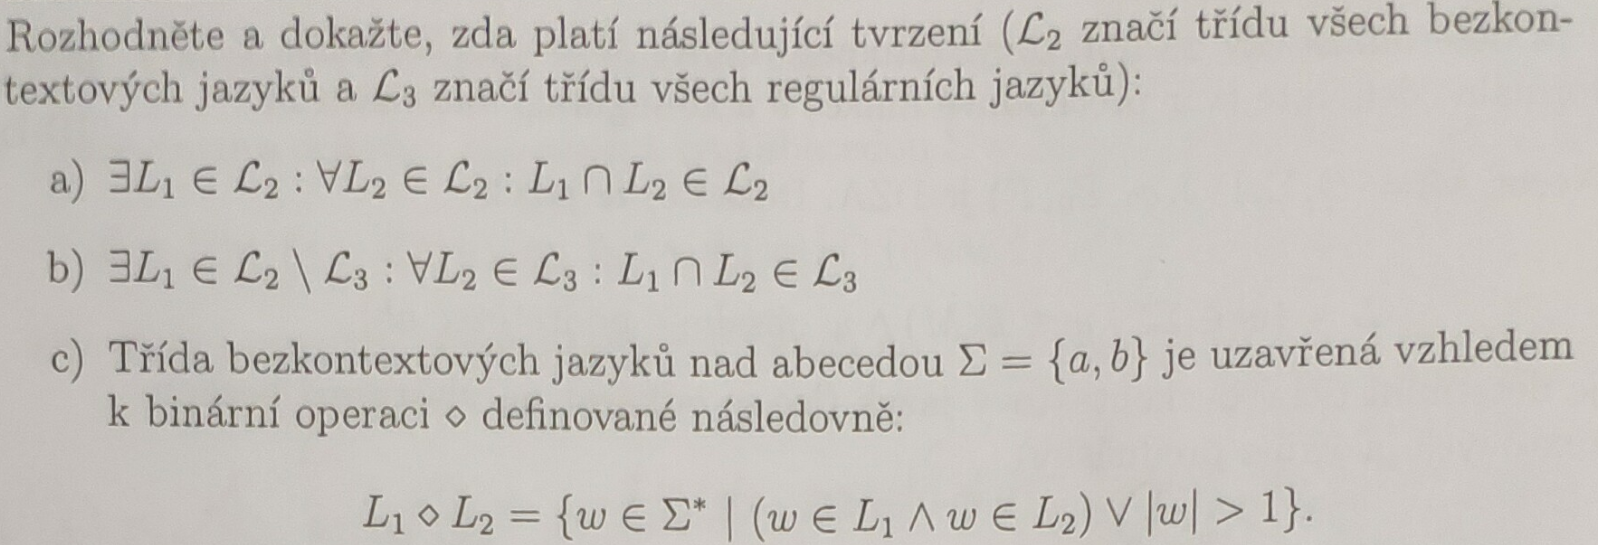
\includegraphics[width=\textwidth]{tasks/vlastnosti/task1.png}
	\end{figure}

	\begin{figure}[H]
		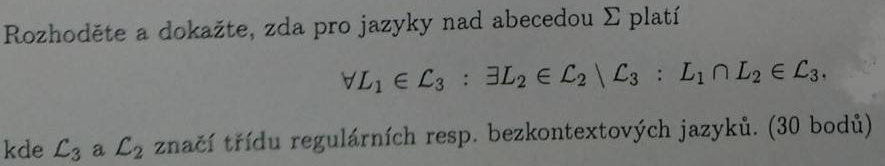
\includegraphics[width=\textwidth]{tasks/vlastnosti/task2.png}
	\end{figure}
	
	\begin{figure}[H]
		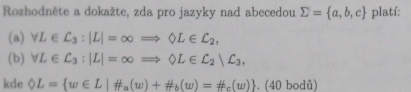
\includegraphics[width=\textwidth]{tasks/vlastnosti/task3.png}
	\end{figure}


	\begin{figure}[H]
		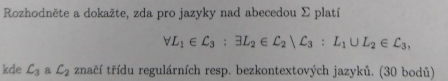
\includegraphics[width=\textwidth]{tasks/vlastnosti/task4.png}
	\end{figure}
	
	\begin{figure}[H]
		
\includegraphics[width=\textwidth]{tasks/vlastnosti/task5.png}
	\end{figure}

	\begin{figure}[H]
		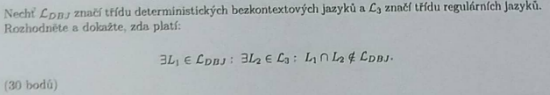
\includegraphics[width=\textwidth]{tasks/vlastnosti/task6.png}
	\end{figure}

	\section{Turingove stroje}
	
	Definicia prechodovej funkcie NTS, retazec prijimany TS, jazyk prijimany TS. TS zadaný prechodovou funkciou mal na vstupu $\Delta$abca$\Delta^{w}$ a bylo třeba doplnit 4 pravidla tak, aby výstup byl $\Delta$acba$\Delta^{w}$.
	
	\begin{figure}[H]
		
\includegraphics[width=\textwidth]{tasks/ts/task1.png}
	\end{figure}

	\begin{figure}[H]
		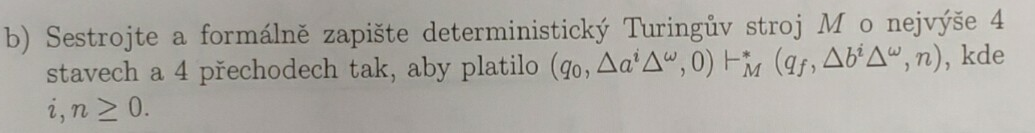
\includegraphics[width=\textwidth]{tasks/ts/task2.png}
	\end{figure}
	
	\section{Diagonalizácia}
	
	\begin{figure}[H]
		
\includegraphics[width=\textwidth]{tasks/diagonalizacia/task1.png}
	\end{figure}

	\begin{figure}[H]
		
\includegraphics[width=\textwidth]{tasks/diagonalizacia/task2.png}
	\end{figure}
	
	\section{Redukcie, rekurzívne a rekurzívne vyčísliteľné jazyky}
	
	\begin{figure}[H]
		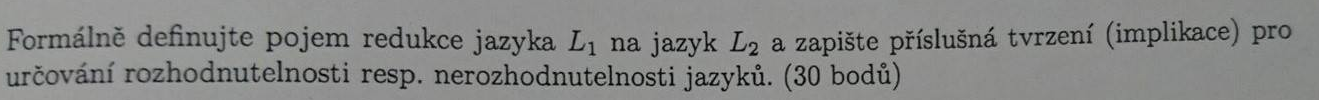
\includegraphics[width=\textwidth]{tasks/redukcie/task1.png}
	\end{figure}

	\begin{figure}[H]
		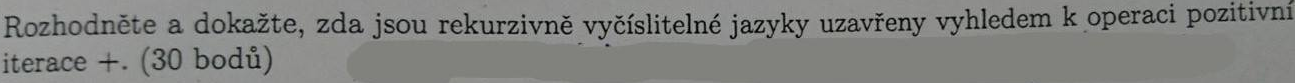
\includegraphics[width=\textwidth]{tasks/redukcie/task2.png}
	\end{figure}
	
	\begin{figure}[H]
		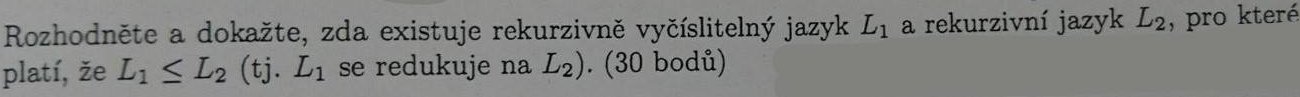
\includegraphics[width=\textwidth]{tasks/redukcie/task3.png}
	\end{figure}
	
	\begin{figure}[H]
		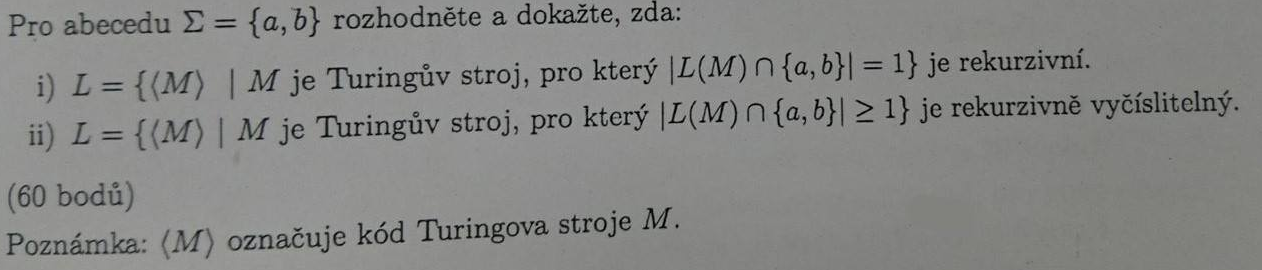
\includegraphics[width=\textwidth]{tasks/redukcie/task4.png}
	\end{figure}

	\begin{figure}[H]
		
\includegraphics[width=\textwidth]{tasks/redukcie/task5.png}
	\end{figure}

	\begin{figure}[H]
		
\includegraphics[width=\textwidth]{tasks/redukcie/task6.png}
	\end{figure}

	\begin{figure}[H]
		
\includegraphics[width=\textwidth]{tasks/redukcie/task7.png}
	\end{figure}
	
	\begin{figure}[H]
		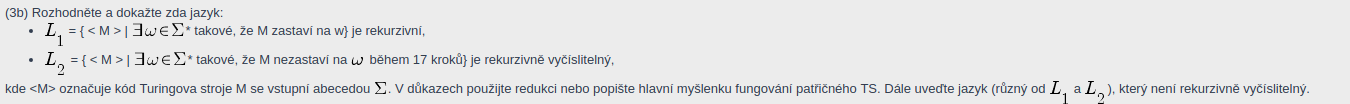
\includegraphics[width=\textwidth]{tasks/redukcie/task8.png}
	\end{figure}
	
	\section{Zložitosť}
	
	\begin{figure}[H]
		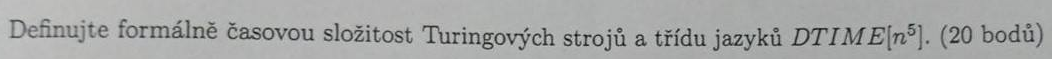
\includegraphics[width=\textwidth]{tasks/zlozitost/task1.png}
	\end{figure}

	\begin{figure}[H]
		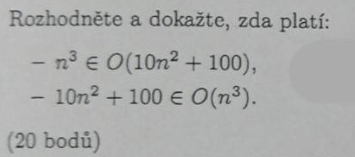
\includegraphics[width=\textwidth]{tasks/zlozitost/task2.png}
	\end{figure}

	\begin{figure}[H]
		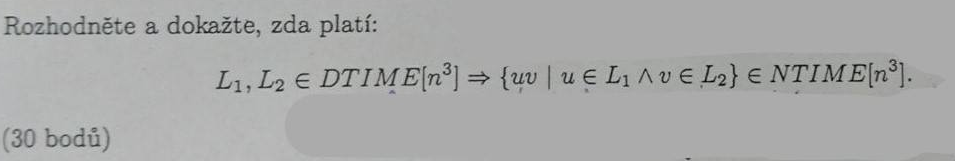
\includegraphics[width=\textwidth]{tasks/zlozitost/task3.png}
	\end{figure}
	
	\begin{figure}[H]
		\includegraphics[width=\textwidth]{tasks/zlozitost/task4.png}
	\end{figure}

	\begin{figure}[H]
		\includegraphics[width=\textwidth]{tasks/zlozitost/task5.png}
	\end{figure}

	\begin{figure}[H]
		\includegraphics[width=\textwidth]{tasks/zlozitost/task6.png}
	\end{figure}
	
	\begin{figure}[H]
		\includegraphics[width=\textwidth]{tasks/zlozitost/task7.png}
	\end{figure}

	\section{NP problémy, polynomiálna redukcia}
	
	\begin{figure}[H]
		\includegraphics[width=\textwidth]{tasks/np/task1.png}
	\end{figure}

	\begin{figure}[H]
		\includegraphics[width=\textwidth]{tasks/np/task2.png}
	\end{figure}
	
	\begin{figure}[H]
		\includegraphics[width=\textwidth]{tasks/np/task3.png}
	\end{figure}

	\section{Vyčíslitelné funkcie}

	\begin{figure}[H]
		\includegraphics[width=\textwidth]{tasks/funkcie/task1.png}
	\end{figure}

	\section{Petriho siete}
	
	\begin{figure}[H]
		\includegraphics[width=\textwidth]{tasks/petri/task1.png}
	\end{figure}

	\begin{figure}[H]
		\includegraphics[width=\textwidth]{tasks/petri/task2.png}
	\end{figure}

	\begin{figure}[H]
		\includegraphics[width=\textwidth]{tasks/petri/task3.png}
	\end{figure}

	
\end{document}